\chapter{Tür und Box}
\section{Herstellung der einzelnen Teile}
\subsection{Türblatt}
Das Türblatt besteht aus einer einzelnen Holzplatte. Die genauen Maße dieser Holzplatte betragen 35x47cm.
Diese Holzplatte wurde aus dem Holzverschnitt einer herkömmlichen Baumarkt-Handelskette erworben. Die Kosten des
Türblatts betrugen 6€.

Es mussten keine weiteren Änderungen am Türblatt vorgenommen werden. Wir entschieden uns,
den Rahmen an das Türblatt anzupassen.

\subsection{Türrahmen}
Um den Türrahmen herzustellen, wurde zuerst weiteres Holz besorgt. Dieses Holzstück hatte bereits weitgehend geeignete Maße.
Es war ein langes Brett, aus dem die vier Seiten des Türrahmens gebildet werden konnten.
Um vom Ausgangsholz bis hin zum fertigen Türrahmen zu gelangen, wurden folgende Schritte getätigt:
\begin{enumerate}
    \item \textbf{Vierkanthobel}: Zuerst wurde das Werkstück an allen vier Seiten gleichzeitig mithilfe eines Vierkanthobels bearbeitet.
    Dadurch wurde die Oberfläche der Werkstücke geglättet und abgerichtet.
    \item \textbf{Stufe schneiden}: Da das Türblatt mit dem Türrahmen bündig sein soll, also ein stumpf einschlagendes Türblatt sein soll,
    muss in den Türrahmen eine Stufe geschnitten werden. Ansonsten würde nichts das Türblatt beim Schließen der Tür stoppen.
    \item \textbf{Zuschneiden}: Als nächstes wurde das Werkstück in vier Teile auf Maß zugeschnitten. Aus Schönheitsgründen wurden die
    Werkstücke in Gehrung geschnitten. Das bedeutet, dass die zwei Eckstücke mit 45° zugeschnitten werden, damit sie dann genau aneinander
    liegen können, wenn sie zu einem Rahmen zusammengeführt werden.
    \item \textbf{Verleimen und Verschrauben}: Die vier Teile des Rahmens wurden nun zusammengeführt und verleimt. Zusätzlich wurden sie mit
    Holzbauschrauben gesichert, um das ganze Konstrukt robuster zu machen.
\end{enumerate}
Der Türrahmen war somit fertig.

\subsection{Holzbox}
Da die Holzbox ein recht kleines Werkstück ist, entschieden wir uns dafür, kleine Sperrholzplatten als Ausgangsmaterial zu verwenden.
Diese Sperrholzplatten hatten die Maße 20x30x0,4cm und waren für die Bearbeitung mit einer Laubsäge geeignet. Wir entschieden uns aus
Genauigkeitsgründen aber gegen die Verwendung einer Laubsäge. Wir entschieden uns für das Verwenden einer Kreissäge.

Die Herstellung der Holzbox kann ebenfalls in einfache Schritte unterteilt werden:
\begin{enumerate}
    \item \textbf{Eroieren der Maße}: Als erstes mussten wir die genauen Maße der Holzbox festlegen. Da das Touchdisplay direkt als
    Vorderseite der Box fungieren soll, mussten wir die Maße auf das Display anpassen. Das Display hat die Maße 19,5*12,5cm.
    \item \textbf{Aufzeichnen der Schnitte}: Bevor wir die Sperrholzplatten zuschneiden konnten, mussten wir natürlich die gewollten
    Schnitte auf das Holz aufzeichnen, um für eine gewisse Genauigkeit zu sorgen. Dies setzten wir mit einem schwarzen Adding-Stift um.
    \item \textbf{Ausschneiden}: Das Ausschneiden mit der Kreissäge war nun ein Kinderspiel. Trotzdem ist beim Arbeiten mit einer Kreissäge
    enorm auf die eigene Sicherheit zu achten.
    \item \textbf{Zusammenleimen}: Nun leimten wir die ausgeschnittenen Teile zu einer Box zusammen. Da die Holzplatten sehr dünn sind,
    machte ein Gehrungsschnitt keinen Sinn. Wir leimten sie normal aufeinander zusammen. Das Ergebnis ist eine Holzbox ohne Boden und Decke.
    Ein Loch für den Touchscreen, das andere um in die Box greifen zu können.
    \item \textbf{Hinzufügen der Klappe}: Um die Box öffnen und schließen zu können, mussten wir noch eine Holzklappe hinzufügen. Das machten
    wir einfach mit einer weiteren Holzplatte. Als Scharnier fungiert hierbei starkes Gewebeklebeband, da es völlig ausreichend ist.
\end{enumerate}

Nun fehlte nur noch das Einsetzen des Touchscreens.


\section{Vollendung der Modelltür}
Zur Vollendung der Modelltür musste nur noch das Zusammenfügen von Türrahmen und Türblatt erfolgen.
Da das Türblatt bündig mit dem Türrahmen ist, ließen sich leicht herkömmliche Scharniere aus Metall als Türscharniere verwenden.

Um die Tür auch ohne Strom schließbar zu machen, haben wir einen kleinen Türriegel hinzugefügt. Alle Komponenten wurden mit
Schrauben auf dem Türrahmen und dem Türblatt befestigt.

Die Modelltür wurde somit erfolgreich produziert.
\begin{figure}[H]
    \begin{center}
        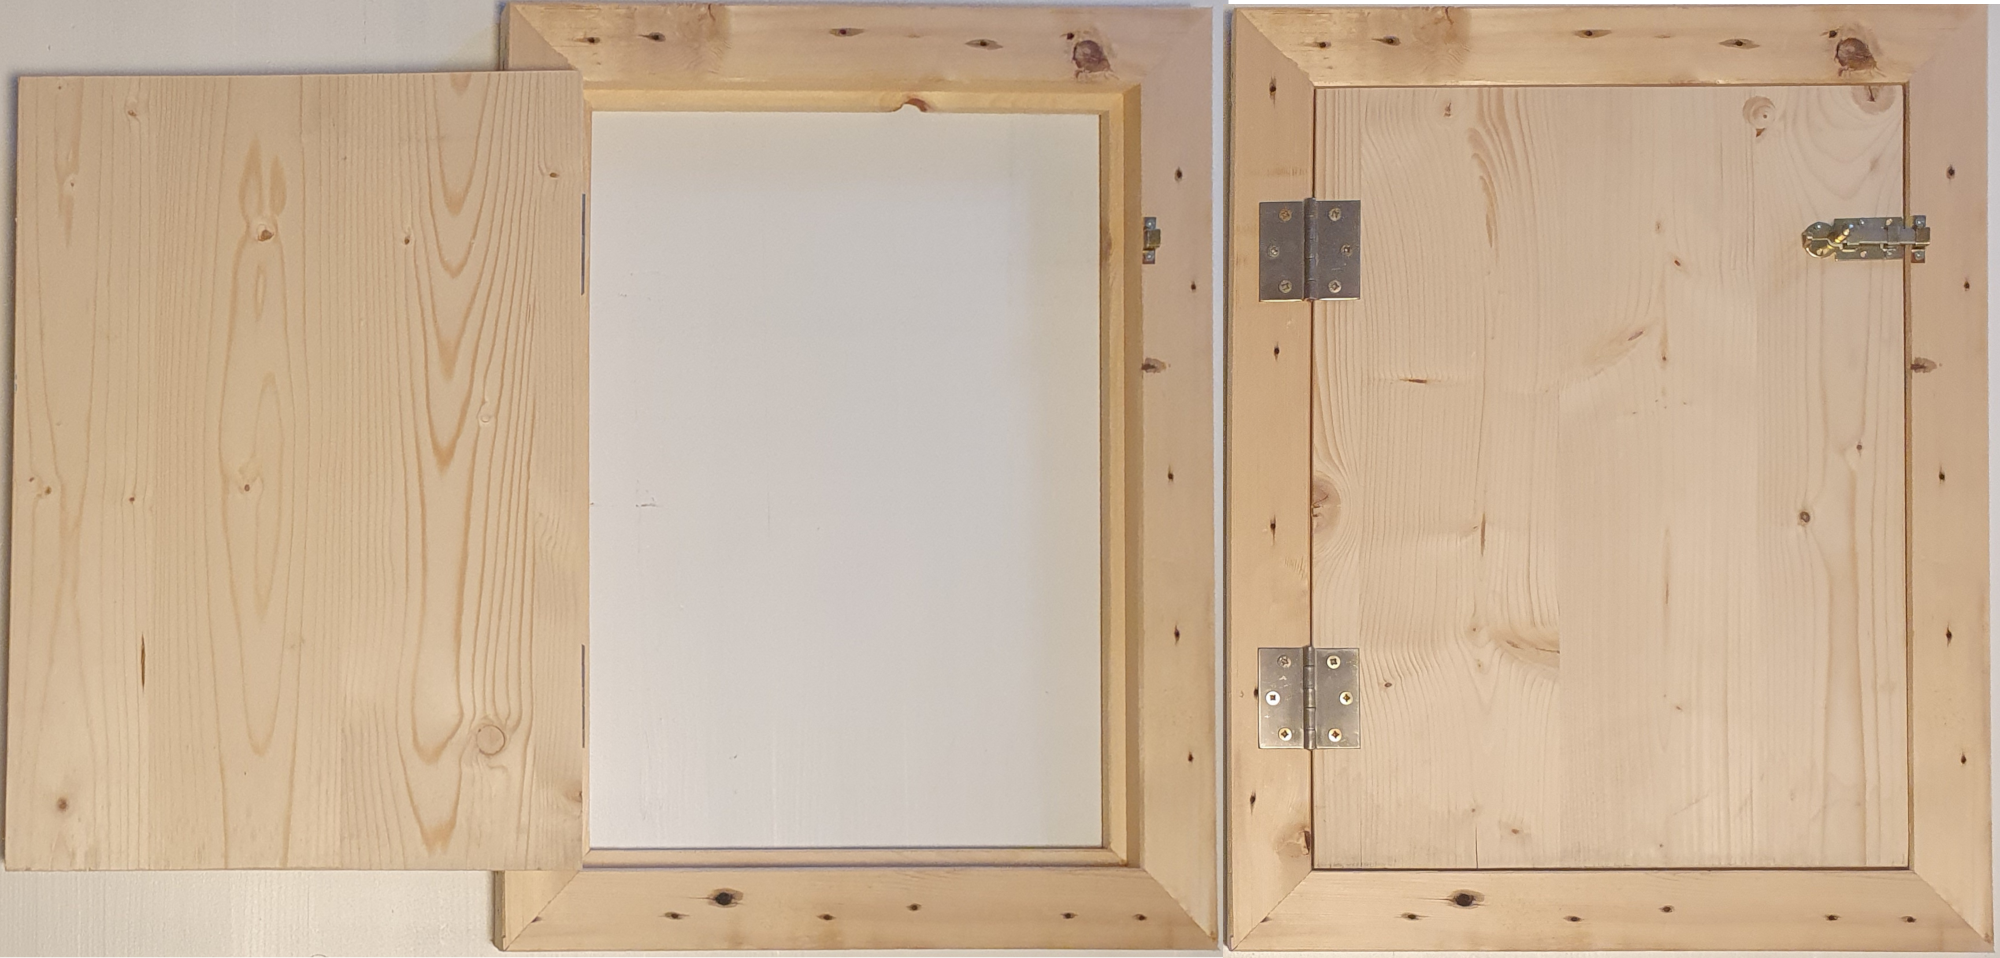
\includegraphics[width=0.9\textwidth]{images/core/tuer_aufzu.png}
        \caption{Modelltür; geöffnet und geschlossen}
    \end{center}
\end{figure}

\section{Vollendung der Holzbox}
Um das Aussehen der Holzbox etwas aufzuschmücken, haben wir schwarzes Klebeband um die Box gewickelt. Dies dient auch zur Verbesserung der
Stabilität. Das Display wurde mithilfe von doppelseitigen Klebeband befestigt. Dies ermöglicht leichtes Wiederabnehmen des Bildschirms.
Das ist äußerst nützlich, falls später noch etwas am Display geändert werden muss.


\begin{figure}[H]
    \begin{center}
        \includegraphics[width=0.9\textwidth]{images/core/box_45innen.jpg}
        \caption{Box in zwei Ansichten}
    \end{center}
\end{figure}